\documentclass[11pt, onecolumn]{article}
% \setlength{\columnsep}{0.2cm}

\usepackage{amssymb}
\usepackage{amsmath}
\usepackage[a4paper, margin=2.5cm]{geometry}
%\usepackage{mathtools}
\usepackage{graphicx}

\usepackage{color}
\usepackage[usenames,dvipsnames,svgnames,table]{xcolor}

\usepackage[colorlinks=true,linkcolor=blue, citecolor=BlueGreen]{hyperref}
%\hypersetup{ pdfborder = {0 0 0}}

\usepackage[parfill]{parskip}
\usepackage{lscape}

\usepackage{xspace}
\usepackage[labelfont=bf,font={small,sl},labelsep=period,justification=raggedright]{caption}

\usepackage{fancyhdr}
\pagestyle{fancy}
\lhead{ }
\rhead{\naf documentation}

%%%%%%%%%%%%%%%%%%%%%%%%

\title{\naf (New Agent-based model for Flu) Documentation}
\author{David Champredon}

%%%%%%%%%%%%%%%%%%%%%%%%

\newcommand{\ttt}[1]{\texttt{#1}}
\newcommand{\one}[1]{\textbf{\large{1}}_{#1}}
\newcommand{\warning}[1]{\textbf{\textcolor{OrangeRed}{#1}}}
\newcommand{\note}[1]{\textit{\textcolor{Grey}{Note: #1}}}
\newcommand{\eg}{\textit{e.g.}\xspace}
\newcommand{\ie}{\textit{i.e.}\xspace}
\newcommand{\etal}{\textit{et al.}\xspace}
\newcommand{\naf}{\textsf{NAF}\xspace}

\newcommand{\immh}{\ensuremath{\text{imm}_h}}
\newcommand{\immc}{\ensuremath{\text{imm}_c}}

%%%%%%%%%%%%%%%%%%%%%%%%
%%%%%%%%%%%%%%%%%%%%%%%%
%%%%%%%%%%%%%%%%%%%%%%%%
%%%%%%%%%%%%%%%%%%%%%%%%

\begin{document}
\maketitle

\vspace{1cm}

\tableofcontents

\newpage

\section{Introduction}

This documentation describes the implementation of an agent-based model, named \naf, designed specifically for the spread of influenza at the population level. 

The implementation of \naf is \emph{not} event driven. Instead, time is divided in relatively coarse ``slices'' that represent relevant epidemiological periods of a day. Within a given time slice, epidemiological events are calculated only \emph{once}. This approximation allows significant computing time saving for an acceptable loss of realism (of course that depends on the size of time slices). Although each individual is uniquely identified, the information of who infects who is omitted for performance (this is optional though; and time of transmission is always recorded to keep track of the generation interval). 


\naf is implemented with a representation of a spatial structure. The fundamental spatial unit is called a ``social place'' which broadly represents any physical place human mix. Because it is preferable to have a limited number of social places types, only the most relevant ones on which data exists are explicitly represented (for example households, schools, workplace, etc. ). A social place type that represents all other types not explicitly modelled is used. 
In order to have a similar hierarchical structure as real world data, social places are gathered in ``area units'', which are themselves gathered in ``regions''.

The programming language for the model is C++. The executable is wrapped in R, mostly for output analysis and debugging.

\section{High-level summary}

\warning{((TO DO))}

\section{Population}

\subsection{Social place}

\naf is implemented with a spatial structure, and its fundamental spatial unit is called a ``social place''. It represents real world locations where individuals may have relevant contacts for disease transmission (\eg households, schools, public transportations, etc). Because all types of such social places cannot be explicitly described in the model, a social place typed ``other'' is used for all other real-world locations.
In order to have a similar hierarchical structure as real world data, social places are gathered in ``area units'', which are themselves gathered in ``regions''.

The size of a social place, that is the number of linked individuals, is pre-specified with a distribution given as an input. The size distribution is typically a histogram taken from national statistics, when available. 




\subsection{Individuals}

Individuals are uniquely identified in the model with an identification number (ID). The modelled features of an individual are its age, immunity to the disease and frailty. Immunity and frailty are modelled as real number between 0 and 1. They determine respectively the risk of acquiring the disease and of hospitalization. Immunity and frailty can be changed by vaccination and  treatment.

These individuals are ``linked'' to social places. A link means that the individual will eventually visit and have contacts in this social place (according to its schedule, see details later).
All individuals are linked to a social place of type ``household''. Link to other social places depends on individuals: for example, all children aged between 3 and 18 years old are linked to a school but none is linked to a workplace (Figure \ref{fig:SP_indiv}). 


\begin{figure}[!ht]
\centering
    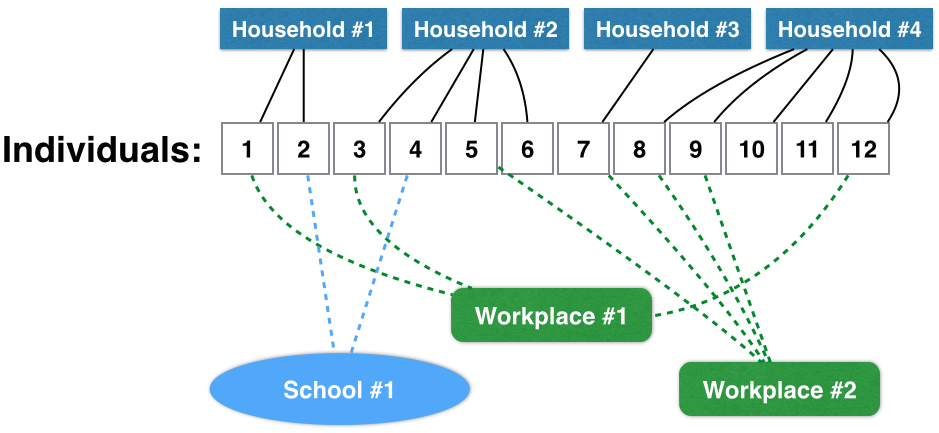
\includegraphics[angle=0,width=0.99\textwidth]{figures/SP_indiv.png}
\caption{Individual and their linked social places. This is a simple illustration of how linkage between individuals and social places is modelled. All individuals are linked to social places of type ``household'' (solid link). Links to other social places depends on the individual's features, like age. For example, individual 1 is an employed adult and hence is linked to a workplace, but not a school.}
\label{fig:SP_indiv}
\end{figure}


\subsection{Population construction}

The world where the simulations will take place is defined iteratively. Briefly, a large number of individuals are created and assigned to households according to the pre-specified distribution of sizes. All households have at least one individual. Once all the households are populated, individuals are assigned an age based on pre-specified age distributions conditional on the household size. For example, a household of size one is associated with an age distribution that has a lower value of 18 years old in order to avoid households populated with only one child. There cannot be an empty household or an individual without a link to a household.

Construction of other social places is more straightforward. The total number of a given social place and its size distribution are pre-specified as inputs. 
Then, individuals are assigned randomly to social places based on individuals' schedule (which is itself base on age, employment rate, etc.). 

If there are not enough social places (of one or more given type), the simulation will eventually fail because individuals that are not linked to a social place that constitutes its schedule (for example a school for a student) will have no determined destination. 


Only social places tagged as ``other'' do not have individuals linked to them, because their purpose is to be visited randomly. 

To summarize, the high level algorithm for the construction of the simulated world is
\begin{enumerate}
\item Create $N_h$ empty households. 
\item Create $N_i$ ageless individuals ($N_i \gg N_h$)
\item Link households with ageless individuals according to the household size distribution
\item Delete superfluous (not linked to an household) ageless individuals 
\item Assign ages to individuals that are linked to an household, based on a pre-specified age distribution given a household size
\item Create social places according to pre-specified number and size distribution
\item Link individuals to social places according to their schedules
\end{enumerate}



\section{Simulator}

\subsection{Model structure}

((write description of compartments and associated flows))

\begin{figure}[!ht]
\centering
    \includegraphics[angle=0,width=0.90\textwidth]{figures/compartments.pdf}
\caption{((write caption!))}
\label{fig:compartments}
\end{figure}


\subsection{Schedules and Spatial movements}

Every individual is assigned a daily ``schedule'' that will determine which social place the individual should visit at a given time of the day. There is a pre-specified probability that the visit actually occurs (based on the individual features, \eg symptomatic infection will reduce the probability \note{not fully implemented yet}).

There is little mixing if an individual would just go back and forth between its household and workplace for example. But social places like ``other'' or ``public transportation'' are supposed to bring some external mixing.


\begin{figure}[!ht]
\centering
    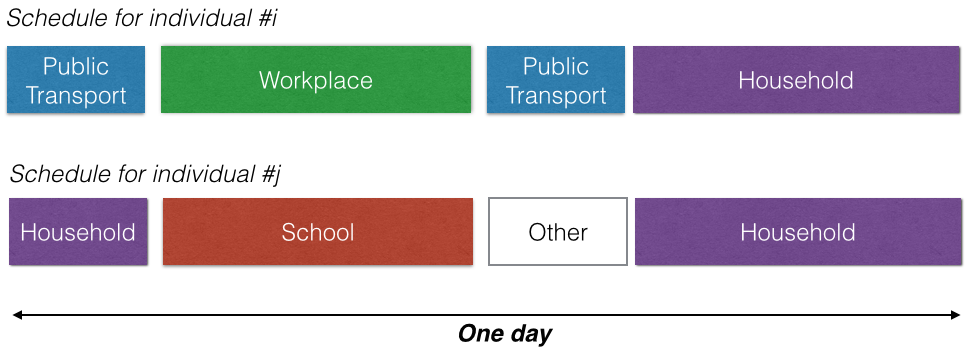
\includegraphics[angle=0,width=0.99\textwidth]{figures/schedule.png}
\caption{Schedules. Simple illustration of different schedules for two individuals. In this example, a day is divided into 4 unequal time slices. Each time slice has the same duration for all individuals, but the social place destination can be different. For example, in this illustration individual $j$ visits its household and school for the first two time slices of the day. Then visit an other social place, randomly chosen. Then finishes the day backin its household.}
\label{fig:SP_indiv}
\end{figure}


\subsection{Transmission process}

Individuals visit a social place during a period that is determined by the time slice of their schedule. During this visit, interaction with other individuals are modelled only if it involves a potential transmission. 

\subsubsection*{Number of contacts}

When an infectious individual is present in a social place, a pre-specified contact rate $r_c$ will determine the number of contacts $n_c$ it will have during its time in that social place. For an individual $i$ in a social place $s$, the contact rate is drawn from a Poisson distribution with a rate itself also drawn from a lognormal distribution. 
\begin{eqnarray}
n_c & \sim & \text{Poisson}(r_c)\\
r_c & \sim & \text{LN}(\lambda(i,s), \sigma)
\end{eqnarray}

The fact the intensity is log-normally distributed allows for super-spreading events. The mean $\lambda$ is parameterized based on the features of individual and of the social place (for example, larger for young ages and in public transports). The standard deviation $\sigma$ is assumed constant.

\subsubsection*{Contacts selection}

Once the number of contacts from an infectious individual is determined, susceptible individuals in this social place are selected randomly as its contacts, with a constraint on age assortativity.

A predefined function specify age assortativity for contacts. More specifically, a function $\phi(x,y)$ gives the likelihood (\emph{not} in the statistical sense) that an individual aged $x$ will contact another individual aged $y$.
In a given social place and for a given number of predetermined contacts, all susceptible individuals are given a ``score'' to be contacted based on the assortativity function $\phi$. 
The higher the score, the more likely the individual will be contacted. The selection is stochastic and a parameter $\lambda$ enables some deviation from the desired assortativity $\phi$.
Indeed, the scores are sorted and the susceptible contact is selected by choosing the rank of the sorted scores from an exponential distribution. If $S_1, S_2, ...$ are the candidate susceptible individuals and $u$ is the indexes vector of the ranked score, the selected susceptible will be $S_{u[X]}$ with $ X \sim \text{Exp}(\lambda) $. The smaller $\lambda$, the more likely that the choice of the susceptible individual will comply to the predefined assortativity function $\phi$.

An example of pre-specified function $\phi$ is shown in Figure \ref{fig:age_assortativity}. A reference for real-world data for $\phi$ is given in Mossong et al \cite{Mossong:2008vz}.


\begin{figure}[!ht]
\centering
    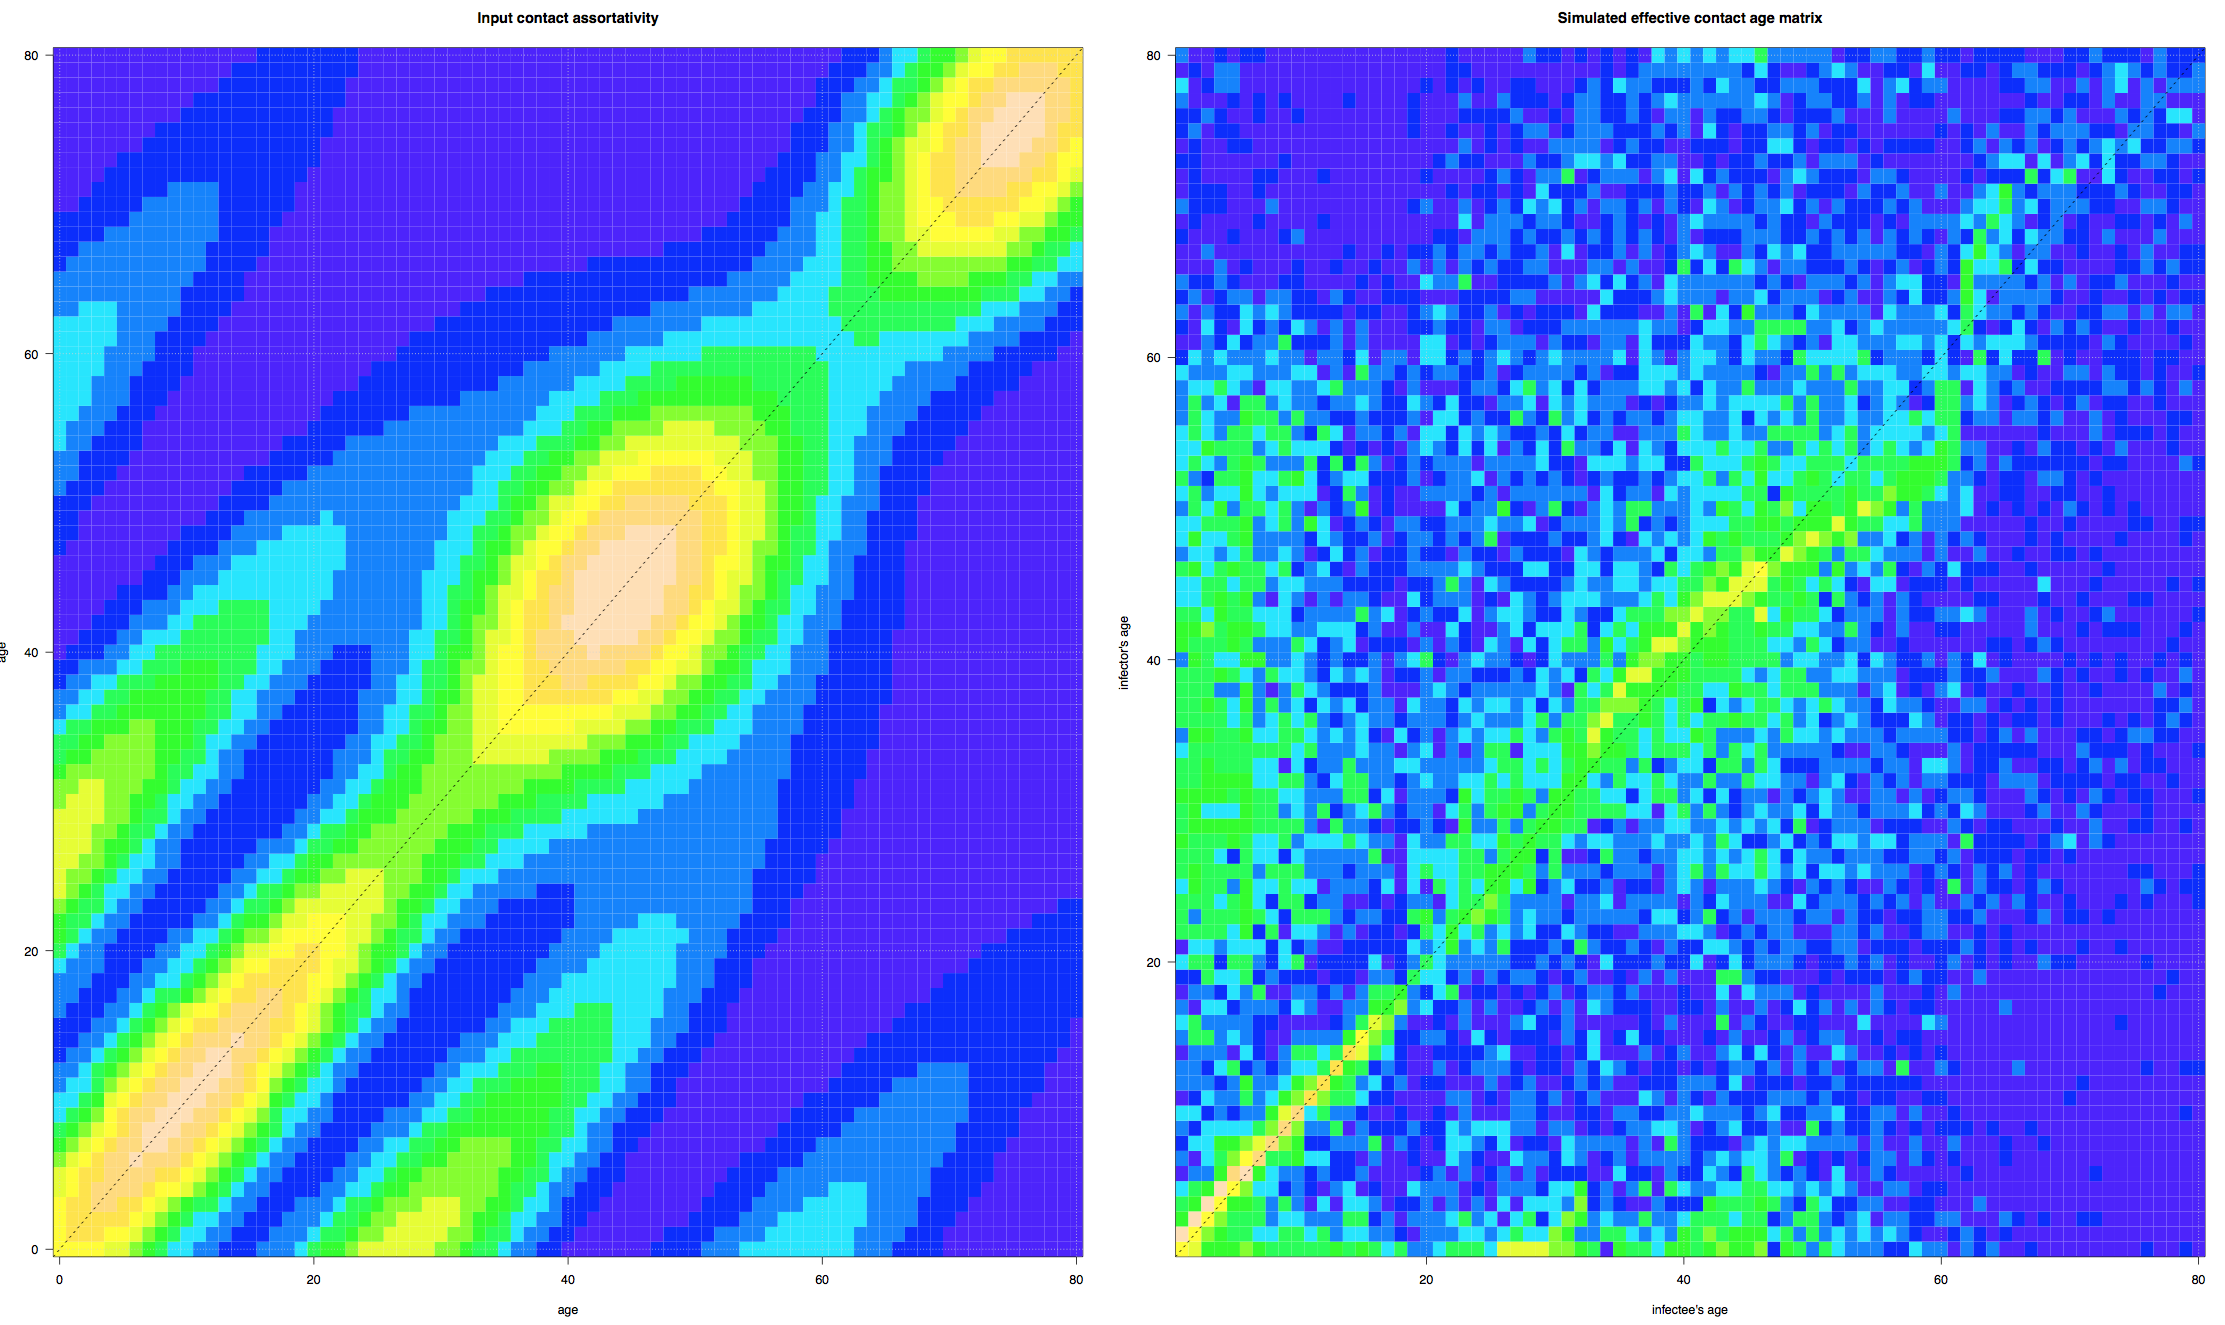
\includegraphics[angle=0,width=0.99\textwidth]{figures/age_assort.png}
\caption{Age assortativity. Example of age assortativity function $\phi$ (left panel) and its realization after a simulation (right panel).}
\label{fig:age_assortativity}
\end{figure}



\subsubsection*{Transmission probabilities}

The probability of actual transmission is the product of two probabilities. The probability the contact from the infectious individual is infectious enough depends on its symptomatic status: a symptomatic infection results in a probability value of 1 (certainty), and an asymptomatic one in a value smaller than one. 

The probability the susceptible contact acquires the disease is based on its \emph{humoral} immunity index $\immh$ which is simply interpreted as the probability infection fails to be established inside the host (thanks to antibodies activity). Humoral immunity is assumed age-dependent. Hence, the probability to acquire infection, conditional on infectious contact is
\begin{equation}
p_{\text{acq}} = 1 - \immh
\end{equation}

The probability the infection will be symptomatic is a function of both frailty $f$ and cellular immunity \immc. Both are age-dependent. The probability of an asymptomatic infection for a susceptible of age $a$ is
\begin{equation}
p_{\text{sympt}} = \immc(a) \, (1-f(a))
\end{equation}

See Figure \ref{fig:transmission}.


\begin{figure}[!ht]
\centering
    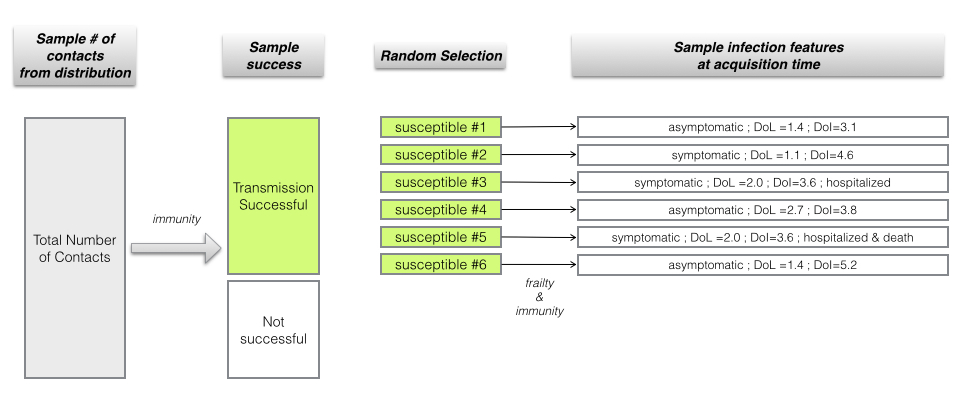
\includegraphics[angle=0,width=0.99\textwidth]{figures/transmission.jpg}
\caption{Transmission. Simplified illustration of the transmission process for an infectious individual in a given social place. DoL: duration of latency; DoI: duration of infectiousness.}
\label{fig:transmission}
\end{figure}


\subsection{Disease progression}

Once a individual has acquired the disease, durations of latency and infectiousness are drawn from a probability distribution. Hospitalization, the duration of hospitalization and disease-induced death are also determined stochastically at acquisition time.
Probabilities to be hospitalized and disease-induced death are based on frailty only.
Deciding these events and durations at acquisition time is more computationally efficient than at each time step of the simulation.

If an individual is hospitalized, it is moved to its linked social place labelled ``hospital'' and stays there for the duration of its hospitalization (movements to other social places directed by its schedule are ignored during hospitalization). Disease-induced death can only occur for hospitalized individuals.


\section{Immunity}

Two types of immunity is modelled: humoral and cell-mediated (``cellular'' hereafter). 

\subsection{Humoral immunity}	
Humoral immunity reflects pre-existing exposure to the pathogen. It is assumed to be the unique determinant of successful infection inside the host. It is modelled as solely age-dependent: decreasing with age (because of immunosenescence).

\begin{equation}
\immh (a) = \frac{H_0 }{a_z}(a_z^p - a^p) ^\frac{1}{p}
\end{equation}
where $a_z$ is the age when humoral immunity reaches 0, $p$ is a shape parameter  and $H_0$ is the baseline.

\note{In the context of pandemic influenza, everyone will have little to no pre-existing exposure, so the baseline humoral immunity $H_0$ has a very low value.}

\begin{figure}[!ht]
\centering
    \includegraphics[angle=0,width=0.90\textwidth]{figures/immunity.pdf}
\caption{Left panel: Example of humoral immunity with $a_z=100$, $H_0=1$ and $p=2$ (thick line) or $p=3$ (thin line). Right panel: Cellular immunity with $\immc^* = 0.7$,  $a_{pivot}=20$ and $s=3$ (thick line) $s=1.5$ (thin line).}
\label{fig:immunity}
\end{figure}

Vaccination has the effect, with a time lag, to increase (by a pre-specified amount) humoral immunity. This results in reducing the likelihood of successful infection (more so once the time lag is passed such that the vaccine has reached its full efficacy). The vaccine-induced increase of humoral immunity is age-dependent as illustrated in Figure \ref{fig:immunity}. 

\subsection{Cellular immunity}	

Cellular immunity is modelled as a determinant of symptomatic infection. It is assumed age-dependent. Because this immunity ``builds up'' through life, older individuals are expected to have a larger cellular immunity than younger ones, hence results in an ``S'' shape curve as illustrated in Figure \ref{fig:immunity}:
\begin{equation}
\immc(a) = \frac{\immc^*}{1+e^{-s(a/a_{pivot} -1)}}
\end{equation}
where $\immc^*$ is the maximum immunity, $s$ and $a_{pivot}$ shape parameters representing the slope and inflection point respectively.

Vaccination has the effect, with a time lag, to increase (by a pre-specified amount) cellular immunity. \warning{investigate this effect and relevant functional shape.}

\section{Interventions}

\subsection{Deployment}

Antiviral treatment and vaccination are implemented as part of ``interventions''. There can be several simultaneous interventions of different nature (\eg vaccination, antiviral treatment).

Any intervention is modelled as having the following features:
\begin{description}
\item[type: ] defines the nature of the intervention: treatment, vaccination, behaviour change.
\item[targeted population:] defines the individuals that can receive the intervention.
\item[time range:] when the intervention begins and ends.
\item[coverage rate:] defines the number of individuals receiving the intervention during a given amount of time
\item[maximum coverage:] specifies if there is a limit to the total number of individuals receiving the intervention.
\end{description}
 
Although the targeted population and roll-out rate are determined deterministically, the actual number of individuals receiving an intervention is stochastic. If $T$ is the total number of individuals targeted to receive the intervention, $r$ is the coverage rate and $dt$ is the simulation time step, then the actual number $N_T$ of individuals receiving the intervention is
\begin{equation}
N_T \sim \text{Poisson}(r\,T\,dt)
\end{equation}

Effect of treatment and vaccination is modelled based on a summary of evidence (see section \ref{sec:antiviral})
Treatment reduces the duration of infection and has no impact on frailty or immunity. Vaccine decreases frailty and increases immunity, both stochastically. The change on both immunity and frailty triggered by vaccination has a (stochastic) time lag and their values change exponentially to the new values drawn at time of vaccination.

\subsection{Treatment effects}

Literature on the effects of antiviral treatment on the course of influenza infection indicates that it marginally reduces the duration of symptoms \warning{((cites))}. It is unclear if antiviral treatment reduces the risk of severe complications, hospitalization or even death. 

Hence, this model implements the effect of antiviral treatment as solely reducing the duration of infection. More specifically, if $d$ is the duration of infection drawn from the pre-specified distribution at infection time, the duration reduction amount $\delta$ is drawn from an exponential distribution: $\delta \sim \text{Exp}(1/\delta^*)$ with $\delta^*$ the pre-specified mean reduction duration. The new (overall) duration of infectiousness at time of treatment initiation is $\max(0, d-\delta)$.

\subsection{Vaccination effects}

Vaccination will potentially increase both humoral and cellular immunities because a reduction of morbidity is observed in vaccinated individuals. However, it is not clear if one is more affected than the other. 

Following vaccination, each individual will have both its humoral and cellular immunity increased by a pre-specified amount. More precisely, the increase of humoral immunity is
\begin{equation}
\immh^{new} = \immh + G_h
\end{equation}
with $G_h$ a gamma distributed random variable with a pre-specified mean $g_h$ and variance $g_h/20$ (a variance 20 times smaller than mean is  only motivated by the resulting distribution shape, see Figure \ref{fig:vax_imm_incr}). 
Similarly, after vaccination the cellular immunity is increased by
\begin{equation}
\immc^{new} = \immc + G_c
\end{equation}
with $G_c$ a gamma distributed random variable with a pre-specified mean $g_c$ and variance $g_c/20$. 
Note that both parameters $g_h$ and $g_c$ are not age-dependent because no literature quantifying this effect was found.

The increase in both immunities is not instantaneous but grows linearly during a pre-specified lag period uniformly distributed between two values around 2 weeks.

Finally, influenza vaccination is assumed to have no effect on individuals' frailty. 

\begin{figure}[!ht]
\centering
    \includegraphics[angle=0,width=0.90\textwidth]{figures/vax_imm_incr.pdf}
\caption{Example of the gamma distribution of additional immunity granted to individuals following vaccination. Mean was set at 0.3.}
\label{fig:vax_imm_incr}
\end{figure}






%%%%%%%%%%%%%%%%%%%%%%%%%%%%%%%%%%%%
%%%%%%%%%%%%%%%%%%%%%%%%%%%%%%%%%%%%
%%%%%%%%%%%%%%%%%%%%%%%%%%%%%%%%%%%%


\newpage
\appendix

\section{Literature review}

\subsection{Influenza natural history}

\textbf{Incubation.} Typically 1-4 days.

\textbf{Viral shedding.} Typically 1 day before symptoms appear. Could be sooner for young children. Shedding sharply reduces after 3-5 days, but could take much longer in young children (up to 10 days after onset) \cite{Carrat:2008bk}. 

\textbf{Recovery.} Typically after 3-7 days after onset.


\subsection{Influenza viral shedding}

Shedding can start about 1 day before symptoms onset, but can even be earlier among young children \cite{CDC:2011wq}. Shedding lasts for several days but is usually sharply reduced by day 3-5 after onset \cite{CDC:2011wq}. The decrease rate is exponential and weak patients experience a slower and longer decrease \cite{Lee:2009dc}.

\begin{figure}[!ht]
\centering
    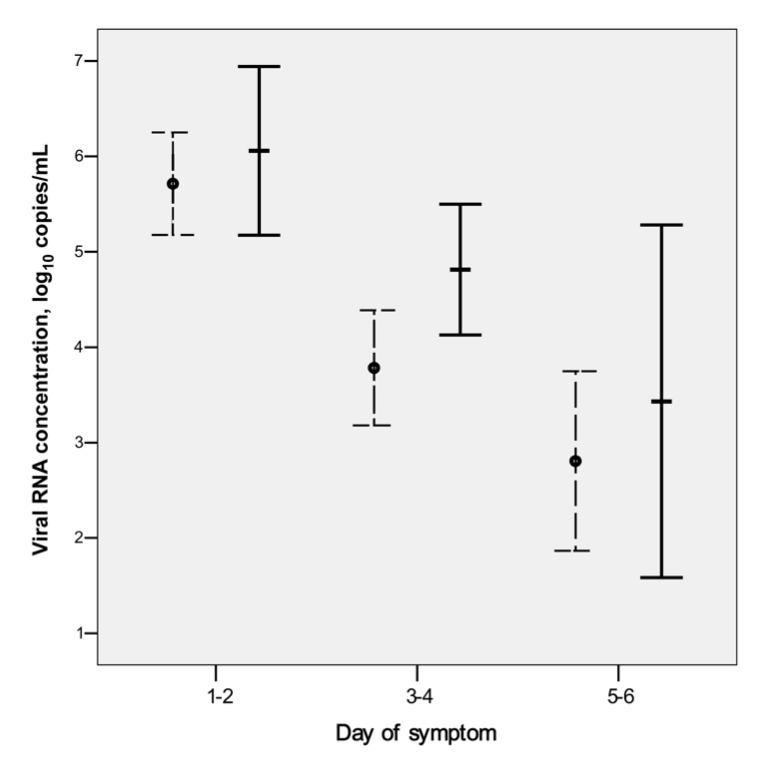
\includegraphics[angle=0,width=0.6\textwidth]{figures/VL_Lee.png}
\caption{Temporal evolution of viral load. Solid lines represent patients with major commorbidities, dashed those without. Source: Lee 2009 \cite{Lee:2009dc}}
\label{fig:VL_Lee}
\end{figure}


\subsection{Influenza-induced hospitalization}

Large majority of children hospitalizations last less than 2 days. Median 3-4 days. Hospitalization mostly occur in young children with pre-existing condition.

Fatality rate in hospital is typically 1-3\% in wealthy countries, but is higher among elderly (6-30\%, but this estimates include poor countries \cite{Wong:2015bb}.


\subsection{Antiviral treatments against Influenza }
\label{sec:antiviral}
Ressources:
\begin{itemize}
\item  CDC recommendations offer a nice overview \cite{CDC:2011wq}.
\item Reviews: Ebell\cite{Ebell:2014ic},  Jefferson 2014 \cite{Jefferson:2014ei}, Jackson 2011 \cite{Jackson:2011ff}
\end{itemize}

Four drugs: 
\begin{itemize}
\item Amantadine and rimantadine: for influenza A only, experience drug resistance.
\item Oseltamivir, Zanamivir: for both influenza A and B, drug resistance rare.
\end{itemize}

Overall, when used on patients already infected, treatment reduces marginally symptoms duration and does not reduce the risk of hospitalization \cite{Ebell:2014ic,Jefferson:2014ei}. 
If administrated within 2 days of onset: reduce duration of uncomplicated illness by 1 day.
If administrated within 1 day of onset: reduce duration of uncomplicated illness by 3.5 days among young children($<3$ years-old) \cite{CDC:2011wq}.

Treatment reduces amount of viral shedding (by how much?) but it's not clear if it reduces the shedding duration.

It is not clear if treatment reduces the risk of severe complications.

Post-exposure chemoprophylaxis is effective at preventing illness (may still be asymptomatic?): 70-90\% reduction in households context. Typical treatment duration: 10 days after most recent contact known \cite{CDC:2011wq}.

Pre-exposure chemoprophylaxis is effective at preventing illness: 80-90\%. Duration of treatment can be as long as 1 month. But because of resistance concerns, pre-exposure chemoprophylaxis is used only for persons at very high risk \cite{CDC:2011wq}. 

Adherence to treatment -- especially for long treatment durations -- is an issue because of side effects.



\subsection{Age and immunity -- Immunosenescence}

Immune response, for both humoral and cellular, decreases quantitatively, as well as qualitatively, with age \cite{Vallejo:2011fe}. In particular, this causes a decreased vaccine response. Some quantification of this decrease on B-cells is provided in \cite{Frasca:2011bj,LeMaoult:1997wf}.


\subsection{Vaccination against Influenza }

Influenza vaccine seems to be effective at reducing disease symptoms and severity, if infected later (probably about 2 weeks because immune response to vaccine takes about this duration to peak \cite{Cox:2004vo}). 
Elderly seem to have a lower immune response to vaccine, but that may be caused by other comorbidities rather than age alone. Infants younger than 6 months may also have a lower immune response to vaccine \cite{Cox:2004vo}.

Influenza vaccine are about 60-100\% effective at reducing morbidity and mortality and about 30-70\% effective at reducing hospitalization of elderly  \cite{Cox:2004vo}.


\section{Computing performances}

(( TO DO))

%%%%%%%%%%%%%%%%%%%%%%%%%%%%%%%%%%%%
%%%%%%%%%%%%%%%%%%%%%%%%%%%%%%%%%%%%
%%%%%%%%%%%%%%%%%%%%%%%%%%%%%%%%%%%%

\newpage

\bibliography{papers}
\bibliographystyle{alpha}

\end{document}




